% Chapter Template

\chapter{Graphical Models: Structural Modeling and Inference} % Main chapter title

\label{Chapter2} % Change X to a consecutive number; for referencing this chapter elsewhere, use \ref{ChapterX}

\lhead{Chapter 2. \emph{Graphical Models: Structural Modeling and Inference}} % Change X to a consecutive number; this is for the header on each page - perhaps a shortened title

\rule{\textwidth}{0.4pt} \\[0.5cm]
\textit{``Study the past if you would define the future."}

\begin{flushright}
Confucius
\end{flushright}
\rule{\textwidth}{0.4pt} 




%----------------------------------------------------------------------------------------
%	SECTION 1
%----------------------------------------------------------------------------------------
\section{Probabilistic Graphical Models}

This chapter     

Graphical models have been studied in many disciplines, such as artificial intelligence \citep{pear_1988}, statistics \citep{lauritzan_1988}.  It is widely considered 
as one of the main progresses in machine learning research by bringing graphs in to assist probabilistic representation, analysis and computing. 


Basically, graphical models are divided into two categories: directed and undirected.  

%-----------------------------------
%	SUBSECTION 1
%-----------------------------------
\subsection{Bayesian Networks}
\begin{definition}
 A Bayesian network is a Directed Acyclic Graph (DAG), which corresponds to a distribution of the form:
 \begin{equation}
  P(X)=\prod_i P(x_i|\text{pa}(x_i))
 \end{equation}
where $X=\cup\{x_i\}$, pa$(x_i)$ denotes the parent nodes of $x_i$. 
\end{definition}

\begin{theorem}
\textbf{D-Separation Rule}:
 Given three non-intersecting subsets of nodes $A,B,S$, in a graph $G$, we consider all possible paths from any node in $A$ to any node in $B$. The path 
is said blocked if either: 
\begin{enumerate}
 \item the path goes through either \emph{head-to-tail} or \emph{tail-to-tail} at the node, and the node is in set $S$, or
 \item the path goes through \emph{head-to-head} at the node, and neither the node nor any of its descendants is in the set $S$. 
\end{enumerate}
If all paths are blocked, then S D-separates $A$ from $B$, and then:
\begin{equation*}
 A\ci B|S
\end{equation*}
\end{theorem}

The D-Separation rule can be simply proofed as follows:
\begin{proof}
	Three type of separating nodes:\emph{tail-to-tail},\emph{head-to-tail} and \emph{head-to-head} are considered in three simple graphs respectively   \\ \\
	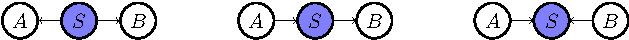
\includegraphics[width=\textwidth]{./Figures/D_Sep}\newline
\begin{minipage}[c]{0.32\textwidth}
 \begin{equation*}
  \begin{array}{rcl}
   & & P(A,B|S)\\
   &=& \frac{P(A,B,S)}{P(S)}\\
   &=& \frac{P(A|S)P(B|S)P(S)}{P(S)}\\
   &=& P(A|S)P(B|S)
  \end{array}
 \end{equation*}
\end{minipage}
\begin{minipage}[c]{0.32\textwidth}
 \begin{equation*}
  \begin{array}{rcl}
   & & P(A,B|S)\\
   &=& \frac{P(A,B,S)}{P(S)}\\
   &=& \frac{P(B|S)P(S|A)P(A)}{P(S)}\\
   &=& P(B|S)\frac{P(S|A)P(A)}{P(S)}\\
   &=& P(B|S)P(A|S)
  \end{array}
 \end{equation*}
\end{minipage}
\begin{minipage}[c]{0.32\textwidth}
 \begin{equation*}
  \begin{array}{rcl}
   & & P(A,B|S)\\
   &=& \frac{P(A,B,S)}{P(S)}\\
   &=& \frac{P(S|A,B)P(A)P(B)}{P(S)}\\
  \end{array}
 \end{equation*}
\end{minipage}\\
\end{proof}

\begin{shaded}
   \textbf{Example:} One morning Tracey found that the grass in her garden is wet ($T\in\{0,1\}$). Is it due to overnight rain ($R \in\{0,1\}$)or did
she forget to turn off the sprinkler last night ($S\in\{0,1\}$)? Next she notices that the grass of her neighbor, Jack, is also
wet ($J\in\{0,1\}$), and she also remembered it was cloudy on the previous daytime ($C\in\{0,1\}$).                   
\end{shaded}

\begin{equation}
 P(J,T,R,C,S)=P(J|R)P(T|R,S)P(R|C)P(C)
\end{equation}

\begin{figure}{t}
   \centering
   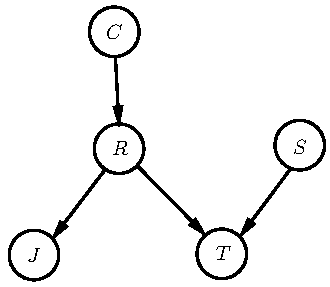
\includegraphics[width=0.4\textwidth]{./Figures/wet_glass_BN.pdf}
   \caption{The Bayesian network corresponding to the wet-glass example.}
\end{figure}

%-----------------------------------
%	SUBSECTION 2
%-----------------------------------
\subsection{Markov Networks}
A more general graph for modeling dependencies among variables is Markov network, or sometimes referred to as Markov random fields (MRFs).      

we can rewrite another factorization form of the joint distribution : 
\begin{equation*}
 \begin{array}{rcl}
   & & P(J,T,R,C,S)\\
   &=& P(J|R)P(T|R,S)P(R|C)P(C)P(S) \\
   &=& \underbrace{P(J|R)}_{\phi_1(J,R)} \underbrace{P(R|C)P(C)}_{\phi_2(R,C)} \underbrace{P(T|R,S)P(S)}_{\phi_3(T,R,S)}\\
   &=& \phi_1(J,R)\phi_2(R,C)\phi_3(T,R,S)
 \end{array}
\end{equation*}
where $\phi_1(J,R), \phi_2(R,C),\phi_3(T,R,S)$ are no longer conditional probabilities

\begin{definition}
 A Markov Network is an undirected graph which corresponds to the distribution of the form:
 \begin{equation}
  P(x_1,x_2,...x_n)=\frac{1}{Z}\prod_{c}\phi_c(X_c)
 \end{equation}
where $X_c$ is a clique of the graph nodes, and $\phi_c(X_c)$ is called potential function over clique $X_c$, and $Z$ is to ensure the distribution normalized.
\end{definition}
\textbf{Remarks:}
\begin{itemize}
 \item the potential function is non-negative, and can be a function of any form over the clique $X_c$, and in most cases it reflects the dependences /compatibilities /constrains among $x_i\in X_c$ ;
 \item the normalization term can be computed as $Z=\sum_{x_1,x_2,...x_n}\prod_{c}\phi_c(X_c)$ or 
 \item the clique defined here means maximal \emph{fully connected subgraph}
\end{itemize}

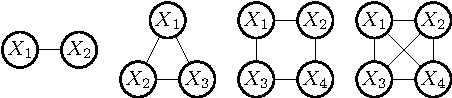
\includegraphics[width=0.9\textwidth]{./Figures/clique}\newline

\begin{minipage}[c]{0.22\textwidth}
 \begin{equation*}
  \psi(X_1,X_2)
 \end{equation*}
\end{minipage}
\begin{minipage}[c]{0.22\textwidth}
 \begin{equation*}
  \psi(X_1,X_2,X_3)
 \end{equation*}
\end{minipage}
\begin{minipage}[c]{0.25\textwidth}
 \begin{equation*}
  \begin{array}{rcl}
   && \psi(X_1,X_2)\\
   && \psi(X_2,X_4)\\
   && \psi(X_1,X_3)\\
   && \psi(X_3,X_4)
  \end{array}
 \end{equation*}
\end{minipage}
\begin{minipage}[c]{0.22\textwidth}
 \begin{equation*}
 \psi(X_1,X_2,X_3,X_4)
 \end{equation*}
\end{minipage}


\begin{theorem}
\textbf{Markov Separation Rule} : a subset $\mathcal{A}$ is said to be separated from another subset $\mathcal{B}$ 
by subset $\mathcal{S}$ if all possible paths from any member of $\mathcal{A}$ to any member $\mathcal{B}$
pass through $\mathcal{S}$. 
 Conditional Independence: If $\mathcal{S}$ separates $\mathcal{A}$ from $\mathcal{B}$, then
 \begin{equation*}
 \mathcal{A} \ci \mathcal{B} | \mathcal{S}
  \end{equation*}
\end{theorem}

\begin{corollary}
\textbf{Local Conditional Independence}:
  when conditioned on its neighbor, $x_i$ is  independent of all other variables of the graph: 
   \begin{equation*}
    P(x_i|X \backslash x_i)= P(x_i|\text{ne}(x_i))
   \end{equation*}
\end{corollary}
For instance,  \newline\newline 
\begin{minipage}[c]{0.5\textwidth}   
	\centering
	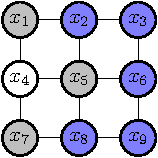
\includegraphics[width=0.5\textwidth]{./Figures/markov_net_1.pdf}
\end{minipage}
\begin{minipage}[c]{0.5\textwidth}
   \begin{equation*}
    x_4 \ci \{x_2,x_3,x_6,x_8,x_9 \}|\{x_1,x_5,x_7\}
   \end{equation*}
\end{minipage}

\begin{corollary}
\textbf{Pairwise Conditional Independence}:
  given two non-adjacent variables $x_i$ and $x_j$ variables, they are independent conditioned all other variables of the graph:
 \begin{equation*}
  x_i \ci x_j | X \backslash \{x_i,x_j\}
 \end{equation*}
\end{corollary}
For instance,  \newline\newline 
\begin{minipage}[c]{0.5\textwidth}   
	\centering
	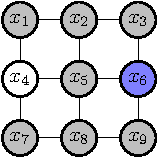
\includegraphics[width=0.5\textwidth]{./Figures/markov_net_2.pdf}
\end{minipage}
\begin{minipage}[c]{0.4\textwidth}
   \begin{equation*}
    x_4 \ci x_6 |\{x_1,x_2,x_3,x_5,x_7,x_8,x_9\}
   \end{equation*}
\end{minipage}


%-----------------------------------
%	SUBSECTION 3
%-----------------------------------
\subsection{Connecting Bayesian Networks and Markov Networks}






%----------------------------------------------------------------------------------------
%	SECTION 2
%----------------------------------------------------------------------------------------
\section{Exact and Approximate Inference}

%-----------------------------------
%	SUBSECTION 1
%-----------------------------------
\subsection{Belief Propagation}

How to compute the probability $P(A)$

\begin{minipage}[c]{0.4\textwidth}
      \centering
      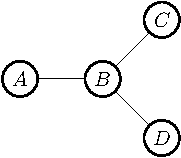
\includegraphics[width=0.75\textwidth]{./Figures/message_passing}
\end{minipage}
\begin{minipage}[c]{0.6\textwidth}
 \begin{equation*}
  \begin{array}{rcl}
  & & P(A) \\
  &=& \overbrace{\sum_{B,C,D}P(A,B,C,D)}^{complexity:  \mathcal{O}(n^{3})} \\
  &\propto& \sum_{B,C,D} \left[ \phi(A,B) \phi(B,C) \phi(B,D) \right] \\
  &\propto& \sum_{B}\phi(A,B) \underbrace{\sum_C \phi(B,C)}_{m_{C\rightarrow B}(B)} \underbrace{\sum_D \phi(B,D)}_{m_{D\rightarrow B}(B)}\\ 
  &\propto& \sum_{B} \left\{\phi(A,B) m_{C\rightarrow B}(B) m_{D\rightarrow B}(B) \right\} \\
  &\propto& m_{B\rightarrow A}(A)
  \end{array}
 \end{equation*}
\end{minipage}

\begin{minipage}[c]{0.4\textwidth}
      \centering
      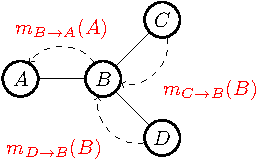
\includegraphics[width=1.1\textwidth]{./Figures/message_passing_1}
\end{minipage}
\begin{minipage}[c]{0.6\textwidth}
 \begin{equation*}
  \begin{array}{rcl}
  & & P(A) \\
  &\propto& \sum_{B}\phi(A,B) \sum_C \phi(B,C) \sum_D \phi(B,D)\\ 
  &\propto& \sum_{B} \left\{\phi(A,B) m_{C\rightarrow B}(B) m_{D\rightarrow B}(B) \right\} \\
  &\propto& m_{B\rightarrow A}(A)
  \end{array}
 \end{equation*}
\end{minipage}\\

\begin{itemize}
 \item $m_{C\rightarrow B}(B)$ is called belief function of $B$ over $C$ by summing out $C$ from the potential function $\sum_C \phi(B,C)$, and it will propagate afterwards; 
 \item intuitively, belief propagation can be understood as a 'message passing scheme', $m_{C\rightarrow B}(B)$ is a message  sent from $C$ to $B$ by telling $B$ all possible states of $C$; and then 
 all messages are processed and passed forward$A$;
\end{itemize}


\begin{minipage}[c]{0.4\textwidth}
      \centering
      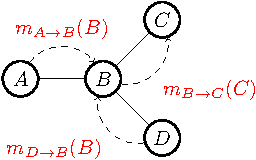
\includegraphics[width=1.1\textwidth]{./Figures/message_passing_2}
\end{minipage}
\begin{minipage}[c]{0.6\textwidth}
 \begin{equation*}
  \begin{array}{rcl}
  & & P(C) \\
  &\propto& \sum_{A}\phi(A,B) \sum_B \phi(B,C) \sum_D \phi(B,D)\\ 
  &\propto& \sum_B \phi(B,C)  \sum_{A}\phi(A,B) \sum_D \phi(B,D)\\ 
  &\propto& \sum_{B} \left\{   \phi(B,C) m_{A\rightarrow B}(B) m_{D\rightarrow B}(B) \right\} \\
  &\propto& m_{B\rightarrow C}(C)
  \end{array}
 \end{equation*}
\end{minipage}

  one variable can send a message to one of its neighbor only if it has received messages from all other variables  
  \begin{equation*}
   m_{B\rightarrow C}(C)=\sum_{B} \left\{   \phi(B,C) m_{A\rightarrow B}(B) m_{D\rightarrow B}(B) \right\}
  \end{equation*}


\begin{minipage}[c]{0.4\textwidth}
      \centering
      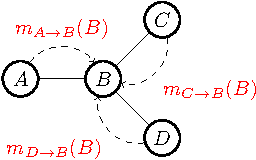
\includegraphics[width=1.1\textwidth]{./Figures/message_passing_3}
\end{minipage}
\begin{minipage}[c]{0.6\textwidth}
 \begin{equation*}
  \begin{array}{rcl}
  & & P(B) \\
  &\propto& \sum_{A}\phi(A,B) \sum_C \phi(B,C) \sum_D \phi(B,D)\\  
  &\propto& m_{A\rightarrow B}(B) m_{C\rightarrow B} (B) m_{D\rightarrow B}(B)  \\
  \end{array}
 \end{equation*}
\end{minipage}\\

 the marginal probabilities are computed as the product of incoming messages:
  \begin{equation*}
  \begin{array}{rcl}
   P(B)&=&\frac{1}{Z}m_{A\rightarrow B}(B) m_{C\rightarrow B} (B) m_{D\rightarrow B}(B)\\
   P(A)&=&\frac{1}{Z}m_{B\rightarrow A}(A) \\
   P(C)&=&\frac{1}{Z}m_{B\rightarrow C}(C) \\
   P(D)&=&\frac{1}{Z}m_{B\rightarrow D}(D) 
  \end{array}
 \end{equation*}

\begin{algorithm}
	\caption{Belief Propagation for tree-structured Markov networks}
	\label{alg:BP_tree}
\begin{algorithmic}[1]
\STATE  select one variable as the root; 
\STATE  starting from all leaves, propagate \emph{beliefs} toward the root as:
\begin{equation*}
m_{i \rightarrow j}(x_j)= \sum_{x_i}\left\{\phi(x_i,x_j) \prod_{k\in \text{Ne}(i)\backslash j} m_{k \rightarrow i}(x_i)\right\}
\end{equation*}
\STATE  when the root receives all messages from its neighbors, then propagate backwards the \emph{``inverse beliefs"} as the step 2;
\STATE  the marginal probability of each variable is computed as: 
\begin{equation*}
P(x_i)\propto \prod_{k\in \text{Ne}(i)} m_{k \rightarrow i}(x_i)
\end{equation*}
where Ne$(i)$ denotes the neighboring variables of $x_i$ in the graph. 
\end{algorithmic}
\end{algorithm}



\begin{algorithm}
	\caption{Generalized Belief Propagation for Loopy Markov networks}
	\label{alg:LBP}
\begin{algorithmic}[1]
%\STATE  In a loopy graph, there is no root and leaves because of loop.
\STATE  initialize all messages $m_{i\rightarrow j}$ in both directions of all connected variables randomly or with a constant value (\emph{e.g.} 1);
\WHILE {all messages converge}
\STATE  update messages as:
\begin{equation*}
  m^{(t+1)}_{i \rightarrow j}(x_j)= \sum_{x_i}\left\{\phi(x_i,x_j) \prod_{k\in \text{Ne}(i)\backslash j} m^{(t)}_{k \rightarrow i}(x_i)\right\}
\end{equation*}
\ENDWHILE
\end{algorithmic}
\end{algorithm}

%-----------------------------------
%	SUBSECTION 2
%-----------------------------------

\subsection{Variational Method}


%-----------------------------------
%	SUBSECTION 3
%-----------------------------------
\subsection{Markov Chain Monte Carlo}
Markov chain Monte Carlo (MCMC) is a family of sampling algorithms, which are designed to generate samples from a target distribution $p(\mathbf{x}), \mathbf{x}\in\mathbb{R}^d$. 
Usually, directly sampling from $p(\mathbf{x})$ is not possible since its density can be arbitrarily complex, however, $p(\mathbf{x})$ can be evaluated up to a normalizing constant:
\begin{equation*}
	p(\mathbf{x})=\frac{\tilde{p}(\mathbf{x})}{\mathbf{Z}}
\end{equation*}

\subsubsection{Metropolis Algorithm}
\begin{itemize}
	\item the proposal distribution is symmetric: $q(\mathbf{x}^*|\mathbf{x}^t)=q(\mathbf{x}^t|\mathbf{x}^*)$;
	\item acceptance probability is: $\mathcal{A}(\mathbf{x}^*;\mathbf{x}^t) = \min\{1, \frac{p(\mathbf{x}^*)}{p(\mathbf{x}^t)}\}$; 
\end{itemize}
It can be seen in the Metropolis algorithm that  $\mathbf{x}^0,\mathbf{x}^1,\cdot, \mathbf{x}^t$ are not independent because successive samples are correlated. Therefore, in practice, real independent 
samples can be obtained by only retraining samples at every $M$ iterations. 

The detailed balance of the Metropolis algorithm can be proof as follows:
\begin{proof}
	\begin{equation}
		\begin{array}{rcl}
			p(\mathbf{x}^t)p(\mathbf{x}^*|\mathbf{x}^t)&=&p(\mathbf{x}^t)\left(q(\mathbf{x}^*|\mathbf{x}^t)\min\{1,\frac{p(\mathbf{x}^*)}{p(\mathbf{x}^t)}\}\right) \\
												       &=& \min\{p(\mathbf{x}^t)q(\mathbf{x}^*|\mathbf{x}^t),q(\mathbf{x}^*|\mathbf{x}^t)p(\mathbf{x}^*) \}  \\
			                                           &=&p(\mathbf{x}^*)q(\mathbf{x}^*|\mathbf{x}^t)\min\{1,\frac{p(\mathbf{x}^t)}{p(\mathbf{x}^*)}\} \\
																											 &\overset{\text{since } q(\mathbf{x}^*|\mathbf{x}^t)=q(\mathbf{x}^t|\mathbf{x}^*)}=& p(\mathbf{x}^*)\left(q(\mathbf{x}^t|\mathbf{x}^*) \min\{1,\frac{p(\mathbf{x}^t)}{p(\mathbf{x}^*)}\} \right) \\
																							  &=& p(\mathbf{x}^*)p(\mathbf{x}^t|\mathbf{x}^*)
	   \end{array}
	\end{equation}
\end{proof}

\begin{algorithm}[t]
	\caption{Metropolis Algorithm}
	\label{alg:LBP}
\begin{algorithmic}[1]
\STATE initialize $\mathbf{x}^0$.
\FOR {$t=0$ to $T-1$}
\STATE generate a sample uniformly from $[0,1]$: $u\sim \mathcal{U}_{[0,1]}$.
\STATE generate a sample from a symmetric proposal distribution: $\mathbf{x}^*\sim q(\mathbf{x}^*|\mathbf{x}^t)$.
\IF {$u<\min\{1,\frac{p(\mathbf{x}^*)}{p(\mathbf{x}^t)}\}$}
\STATE $\mathbf{x}^{t+1}=\mathbf{x}^*$.
\ELSE 
\STATE $\mathbf{x}^{t+1}=\mathbf{x}^t$.
\ENDIF
\ENDFOR
\end{algorithmic}
\end{algorithm}

\subsubsection{Metropolis-Hasting Algorithm} 
\begin{itemize}
	\item the proposal distribution can be arbitrary (no symmetric restriction): $q(\mathbf{x}^*|\mathbf{x}^t)$;
	\item acceptance probability is: $\mathcal{A}(\mathbf{x}^*;\mathbf{x}^t) = \min\{1, \frac{p(\mathbf{x}^*)q(\mathbf{x}^t|\mathbf{x}^*)}{p(\mathbf{x}^t)q(\mathbf{x}^*|\mathbf{x}^t)}\}$; 
\end{itemize}
\begin{algorithm}[t]
	\caption{Metropolis-Hasting (MH) Algorithm}
	\label{alg:LBP}
\begin{algorithmic}[1]
\STATE initialize $\mathbf{x}^0$.
\FOR {$t=0$ to $T-1$}
\STATE generate a sample uniformly from $[0,1]$: $u\sim \mathcal{U}_{[0,1]}$.
\STATE generate a sample $\mathbf{x}^*\sim q(\mathbf{x}^*|\mathbf{x}^t)$.
\IF {$u<\min\{1,\frac{p(\mathbf{x}^*)q(\mathbf{x}^t|\mathbf{x}^*)}{p(\mathbf{x}^t)q(\mathbf{x}^*|\mathbf{x}^t)}$}
\STATE $\mathbf{x}^{t+1}=\mathbf{x}^*$.
\ELSE 
\STATE $\mathbf{x}^{t+1}=\mathbf{x}^t$.
\ENDIF
\ENDFOR
\end{algorithmic}
\end{algorithm}



The detailed balance of the Metropolis algorithm can be proof as follows:
\begin{proof}
	\begin{equation}
		\begin{array}{rcl}
			p(\mathbf{x}^t)p(\mathbf{x}^*|\mathbf{x}^t)&=&p(\mathbf{x}^t)\left(q(\mathbf{x}^*|\mathbf{x}^t)\min\{1,\frac{p(\mathbf{x}^*)q(\mathbf{x}^t|\mathbf{x}^*)}{p(\mathbf{x}^t)q(\mathbf{x}^*|\mathbf{x}^t)}\}\right) \\
												       &=& \min\{p(\mathbf{x}^t)q(\mathbf{x}^*|\mathbf{x}^t),q(\mathbf{x}^*|\mathbf{x}^t)p(\mathbf{x}^*) \}  \\
			                                           &=& p(\mathbf{x}^*)q(\mathbf{x}^t|\mathbf{x}^*)\min\{1,\frac{p(\mathbf{x}^t)q(\mathbf{x}^*|\mathbf{x}^t)}{p(\mathbf{x}^*)q(\mathbf{x}^t|\mathbf{x}^*)}\} \\
										&=& p(\mathbf{x}^*)\left(q(\mathbf{x}^t|\mathbf{x}^*)\min\{1,\frac{p(\mathbf{x}^t)q(\mathbf{x}^*|\mathbf{x}^t)}{p(\mathbf{x}^*)q(\mathbf{x}^t|\mathbf{x}^*)}\}\right) \\
													   &=& p(\mathbf{x}^*)p(\mathbf{x}^t|\mathbf{x}^*)
	   \end{array}
	\end{equation}
\end{proof}

\subsubsection{Gibbs Sampling Algorithm}
The Gibbs sampling is a special case of MH with the proposal distribution defined as the cyclic conditional distributions among $\{x_1,x_2,\cdots,x_d\}$.               
\begin{algorithm}[t]
	\caption{Gibbs Sampling Algorithm}
	\label{alg:LBP}
\begin{algorithmic}[1]
\STATE initialize $\mathbf{x}^0$.
\FOR {$t=0$ to $T-1$}
\STATE randomly select   
\STATE sample $x^*_k$ from  $p(x_k^*|x_{[1,\cdots,d]/k}^t)$.
\STATE $x^{t+1}_k=x^*_k$.
\ENDFOR
\end{algorithmic}
\end{algorithm}


\begin{itemize}
	\item the proposal distribution: $q(\mathbf{x}^*|\mathbf{x}^t)=p(x_k^*|x_{[1,\cdots,d]/k}^t)$;
	\item acceptance probability is: 
		\begin{equation*}
			\begin{array}{rcl}
				\mathcal{A}(\mathbf{x}^*;\mathbf{x}^t) &=& \min\{1, \frac{p(\mathbf{x}^*)q(\mathbf{x}^t|\mathbf{x}^*)}{p(\mathbf{x}^t)q(\mathbf{x}^*|\mathbf{x}^t)}\} \\
																				  &=& \min\{1, \frac{p(\mathbf{x}^*)p(x_{[1,\cdots,d]/k}^t|x_k^*)}{p(\mathbf{x}^t)p(x_k^*|x_{[1,\cdots,d]/k}^t)}\} \\
															 &=& \min\{1,\frac{p(x_k^*)p()p(x_{[1,\cdots,d]/k}^t|x_k^*)}{p(\mathbf{x}^t)p(x_k^*|x_{[1,\cdots,d]/k}^t)}\} \}
        	\end{array}
	    \end{equation*}
\end{itemize}

%----------------------------------------------------------------------------------------
%	SECTION 3
%----------------------------------------------------------------------------------------
\section{3D Part-Based Shape Modeling with Spatial Latent Dirichlet Markov Random Fields}
\begin{shaded}
{\Huge VI.} \textbf{Hanchen Xiong}, Sandor Szedmak, Justus Piater. {\it 3D Object Class Geometry Modeling with Spatial Latent Dirichlet Markov Random Fields}, In Proceedings of the 35th German Conference on Pattern Recognition (GCPR13), pp 51-60, 2013,  Springer.  
\vspace{-.2cm}

\end{shaded}
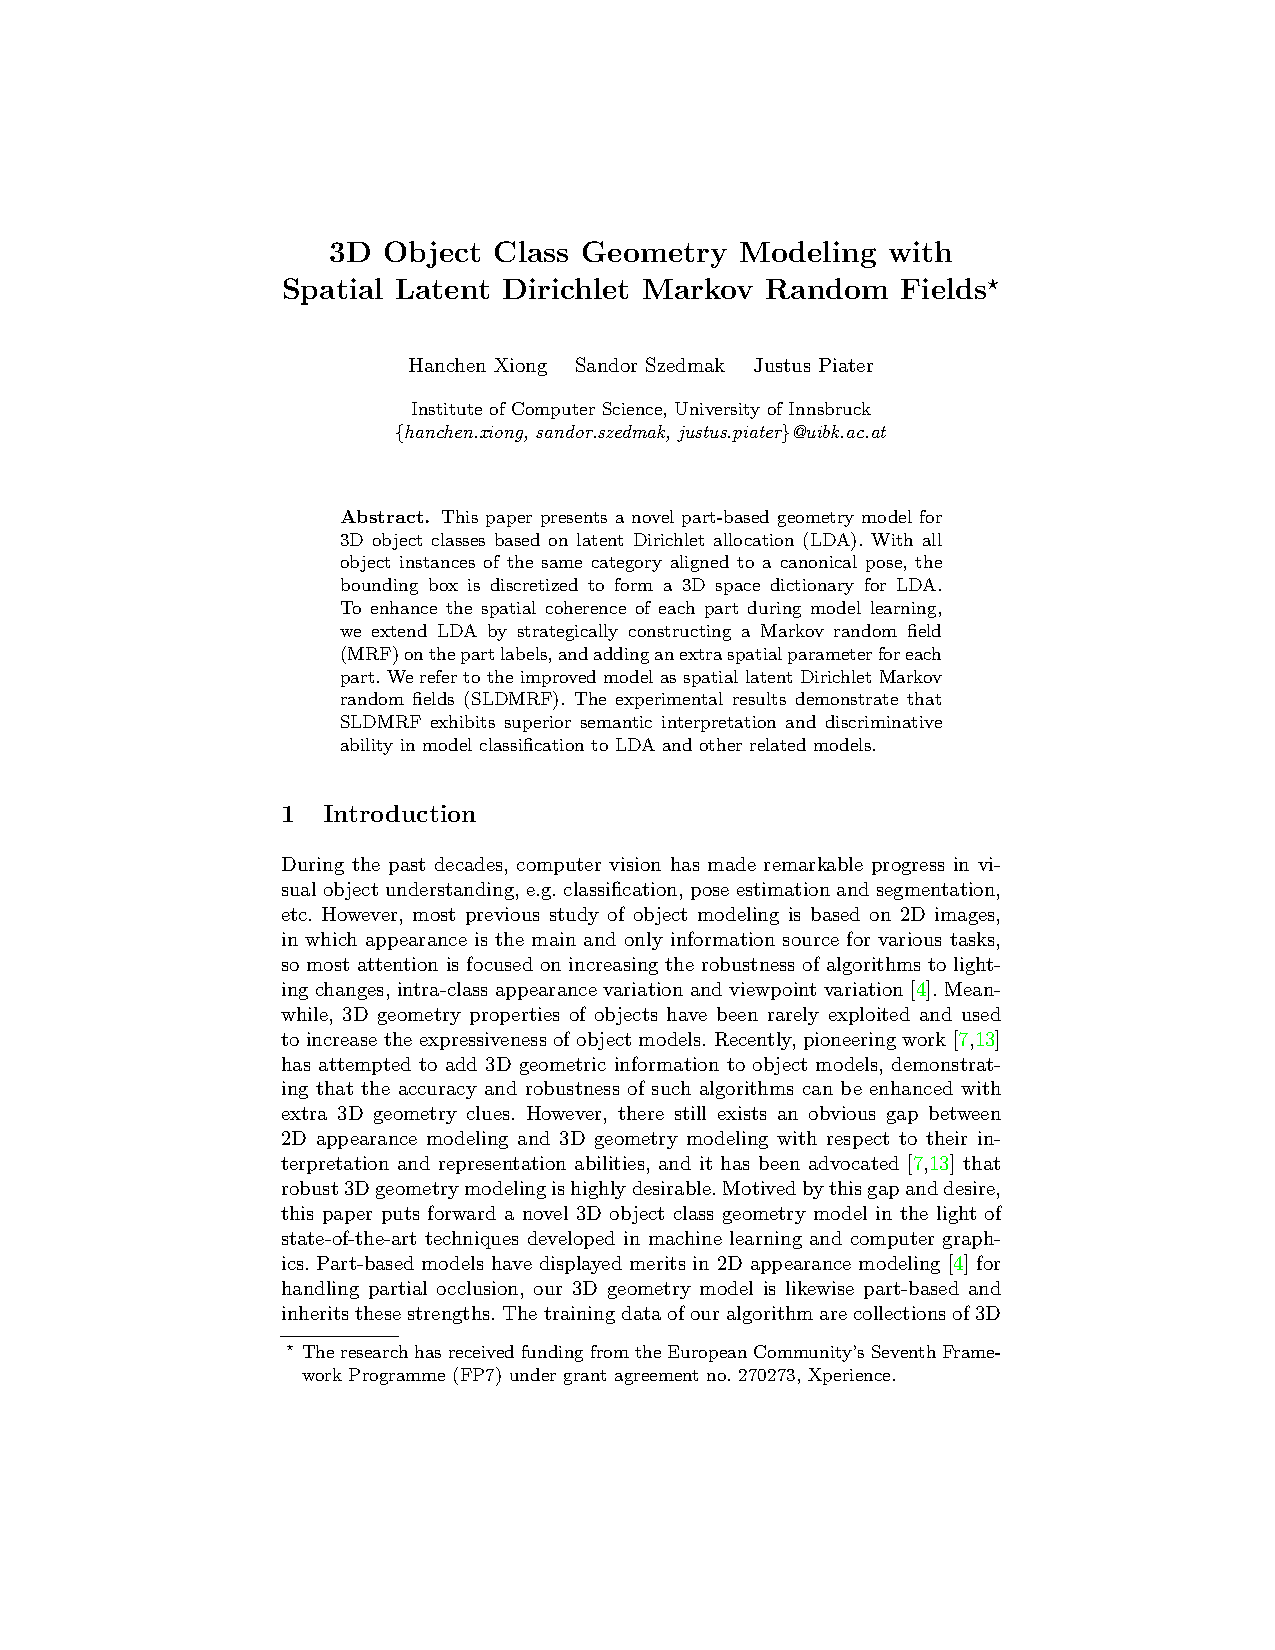
\includepdf[offset=3cm -2.5cm, scale=1.2, pages=-,pagecommand={\pagestyle{fancy}}]{./Papers/Xiong-2013-GCPR.pdf}
